\documentclass{standalone}

\usepackage{graphicx,calc,epstopdf,tikz}

\graphicspath{{./figs/}}

\newlength{\tikzunit}
\setlength{\tikzunit}{\textwidth/16}
\newcommand{\compx}[1]{\textbf{#1}}

\begin{document}
\begin{tikzpicture}[scale=1.0,x=\tikzunit,y=\tikzunit]
    % ---- Draw a grid which should help to position things -----------
    %\draw[step= .20,color=gray,very thin] (-4.95,-4.95) grid ( 4.95, 4.95);
    %\draw[step=1.0,color=gray]            (-4.95,-4.95) grid ( 4.95, 4.95);
    %\draw[step=5.0,color=black]           (-4.95,-4.95) grid ( 4.95, 4.95);
    %  Notes:
    %       just uncomment the lines with draw commands and the grid
    %       will appear.  The commands, I believe are self explanatory
    %       and it can be drawn as big as you want. The two coordinates
    %       denote lower left and upper right corners of the grid.
    % -----------------------------------------------------------------
    \node(0,0){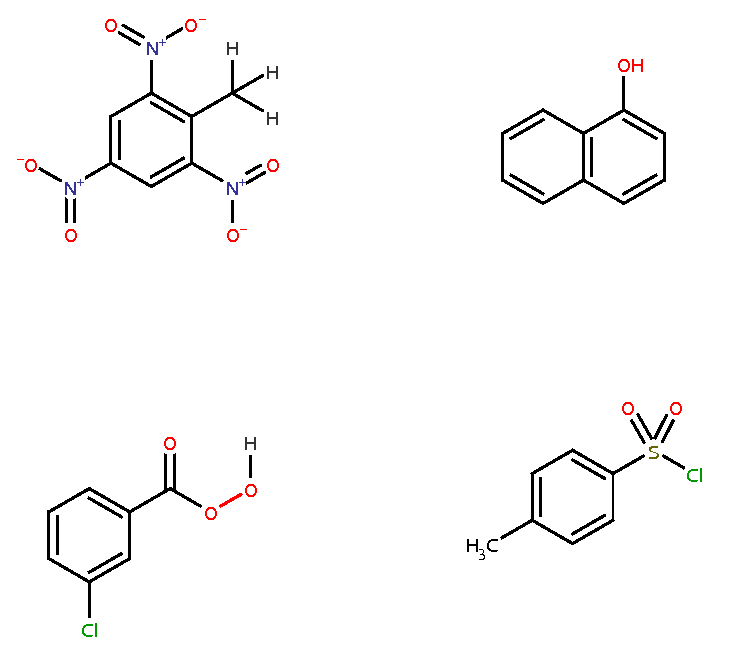
\includegraphics[width=9\tikzunit]{4struct.eps}};
    \draw (-2.8, 1.0) node{TNT};
    \draw ( 2.6, 1.0) node{Naphtol};
    \draw (-2.8,-4.0) node{\compx{1}};
    \draw ( 2.6,-4.0) node{\compx{2}};
\end{tikzpicture}
\end{document}
